%%%%%%%%%%%%%%%%%%%%%%%%%%%%%%%%%%%%%%%%%
% Short Sectioned Assignment
% LaTeX Template
% Version 1.0 (5/5/12)
%
% This template has been downloaded from:
% http://www.LaTeXTemplates.com
%
% Original author:
% Frits Wenneker (http://www.howtotex.com)
%
% License:
% CC BY-NC-SA 3.0 (http://creativecommons.org/licenses/by-nc-sa/3.0/)
%
%%%%%%%%%%%%%%%%%%%%%%%%%%%%%%%%%%%%%%%%%

%----------------------------------------------------------------------------------------
%	PACKAGES AND OTHER DOCUMENT CONFIGURATIONS
%----------------------------------------------------------------------------------------

\documentclass[paper=a4, fontsize=11pt]{scrartcl} % A4 paper and 11pt font size

\usepackage[pdftex]{graphicx}     

\usepackage[T1]{fontenc} % Use 8-bit encoding that has 256 glyphs
\usepackage{fourier} % Use the Adobe Utopia font for the document - comment this line to return to the LaTeX default
\usepackage[english]{babel} % English language/hyphenation
\usepackage{amsmath,amsfonts,amsthm} % Math packages

\usepackage{xcolor}
\usepackage{listings}

\usepackage{url}

\usepackage{sectsty} % Allows customizing section commands
\allsectionsfont{\centering \normalfont\scshape} % Make all sections centered, the default font and small caps

\usepackage{fancyhdr} % Custom headers and footers
\pagestyle{fancyplain} % Makes all pages in the document conform to the custom headers and footers
\fancyhead{} % No page header - if you want one, create it in the same way as the footers below
\fancyfoot[L]{} % Empty left footer
\fancyfoot[C]{} % Empty center footer
\fancyfoot[R]{\thepage} % Page numbering for right footer
\renewcommand{\headrulewidth}{0pt} % Remove header underlines
\renewcommand{\footrulewidth}{0pt} % Remove footer underlines
\setlength{\headheight}{13.6pt} % Customize the height of the header

\numberwithin{equation}{section} % Number equations within sections (i.e. 1.1, 1.2, 2.1, 2.2 instead of 1, 2, 3, 4)
\numberwithin{figure}{section} % Number figures within sections (i.e. 1.1, 1.2, 2.1, 2.2 instead of 1, 2, 3, 4)
\numberwithin{table}{section} % Number tables within sections (i.e. 1.1, 1.2, 2.1, 2.2 instead of 1, 2, 3, 4)

\setlength\parindent{0pt} % Removes all indentation from paragraphs - comment this line for an assignment with lots of text

%----------------------------------------------------------------------------------------
%	TITLE SECTION
%----------------------------------------------------------------------------------------

\newcommand{\horrule}[1]{\rule{\linewidth}{#1}} % Create horizontal rule command with 1 argument of height

\title{	
\normalfont \normalsize 
\textsc{UGR, ETSIIT} \\ [25pt] % Your university, school and/or department name(s)
\horrule{0.5pt} \\[0.4cm] % Thin top horizontal rule
\huge Developement of a power grid ontology and a sample application \\ % The assignment title
\horrule{2pt} \\[0.5cm] % Thick bottom horizontal rule
}

\author{Felipe Oehrwald, Clemens von Schwerin} % Your name

\date{\normalsize\today} % Today's date or a custom date

\begin{document}

\maketitle % Print the title

\section{Ontology details}

The power grid ontology is aimed to give a basis for representing power grids in terms of power production, consumption and transmission. For that purpose the following classes, as listed in figure \ref{fig:classes} were designed.
The most basic building blocks are the \textit{NetworkEntities} which model all physical entities 
a network may consist of and are disjoint. There are \textit{Producers} adding power to the network, \textit{Consumers} drawing energy from the network, \textit{TransportEntities} transporting the energy between exactly two other network entities and \textit{Transformers} managing splits, merges and changes in the transmission type of \textit{TransportEntities}. \\
Those transmission types are modelled in the \textit{TransmissionType} class. This class is divided into two disjoint subclasses \textit{ACTransmission} for alternating current and \textit{DCTransmission} for direct current. \\
Each \textit{TransportEntity} furthermore has a \textit{CableType} indicating the layout of a power line. There are 3 disjoint alternatives: regular \textit{TransmissionLines}, \textit{UndergroundCables} and \textit{UnderseaCables}. \\
Finally every \textit{NetworkEntity} is part of a specific \textit{Network}.

\begin{figure}
\centering
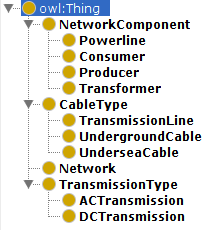
\includegraphics[scale=.75]{img/classes.png} 
\label{fig:classes}
\caption{Class hierarchy of the Power Grid ontology.}
\end{figure}

\bibliographystyle{plain}
\bibliography{documentation}

\end{document}